\subsection{Ports}
\label{sec:wrc_ports}

%\begin{figure}[ht]
%  \begin{center}
%    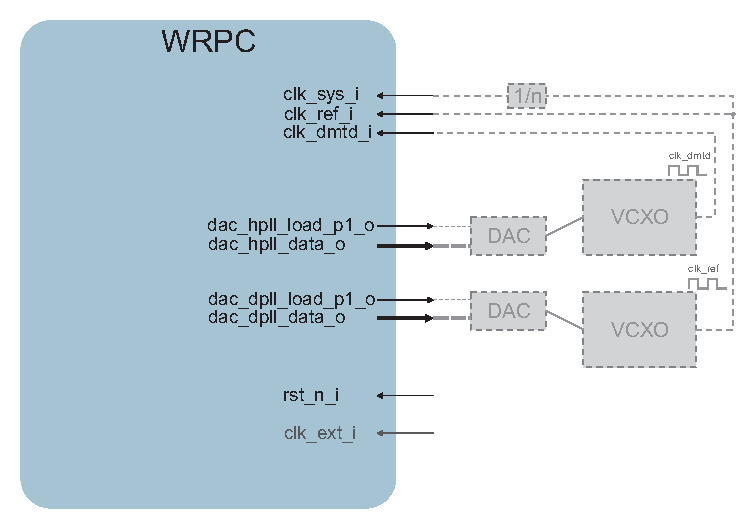
\includegraphics[width=.8\textwidth]{fig/basic_wrpc_clk.pdf}
%    \caption{Mandatory clock signals and main reset of WRPC}
%  \end{center}
%\end{figure}

\begin{hdlporttable}
  \hdltablesection{Clocks and resets}\\
  \hline
  clk\_sys\_i & in & 1 & main system clock, can be any frequency $\leq f_{clk\_ref\_i}$
  e.g. 62.5~MHz\\
  \hline
  clk\_dmtd\_i & in & 1 & DMTD offset clock (close to 62.5 MHz, e.g. 62.49 MHz)\\
  \hline
  clk\_ref\_i & in & 1 & 125 MHz reference clock\\
  \hline
  clk\_aux\_i & in & var & [optional] vector of auxiliary
  clocks that will be disciplined to WR timebase. Size is equal to \tts{g\_aux\_clks}\\
  \hline
  clk\_ext\_mul\_i & in & 1 & 125 MHz clock, derived from \tts{clk\_ext\_i}\\
  \hline
  clk\_ext\_mul\_locked\_i & in & 1 & PLL locked indicator for \tts{clk\_ext\_mul\_i}\\
  \hline
  clk\_ext\_stopped\_i & in & 1 & PLL stopped indicator for \tts{clk\_ext\_mul\_i}\\
  \hline
  clk\_ext\_rst\_o & out & 1 & Reset output to be used for \tts{clk\_ext\_mul\_i}\\
  \hline  
  clk\_ext\_i & in & 1 & [optional] external 10 MHz reference clock input for
  GrandMaster mode\\
  \hline
  pps\_ext\_i & in & 1 & [optional] external 1-PPS input used in GrandMaster mode\\
  \hline
  rst\_n\_i & in & 1 & main reset input, active-low (hold for at least 5
  \tts{clk\_sys\_i} cycles)\\
  \hline
  \hdltablesection{Timing system}\\
  \hline
  dac\_hpll\_load\_p1\_o & out & 1 & validates DAC value on data port \\
  \hline
  dac\_hpll\_data\_o & out & 16 & DAC value for tuning helper (DMTD) VCXO\\
  \hline
  dac\_dpll\_load\_p1\_o & out & 1 & validates DAC value on data port \\
  \hline
  dac\_dpll\_data\_o & out & 16 & DAC value for tuning main (ref) VCXO\\
  \hline
  \hdltablesection{PHY inteface (when \tts{g\_records\_for\_phy = false})}\\
  \hline
  phy\_ref\_clk\_i & in & 1 & TX clock\\
  \hline
  phy\_tx\_data\_o & out & var & TX data. If \tts{g\_pcs\_16bit = true}, then \tts{size = 16}, else \tts{size=8}\\
  \hline
  phy\_tx\_k\_o & out & var & \tts{1} when \tts{phy\_tx\_data\_o} contains a control code, \tts{0} when it's a data byte. If \tts{g\_pcs\_16bit = true}, then \tts{size = 2}, else \tts{size=1}\\
  \hline
  phy\_tx\_disparity\_i & in  & 1 & disparity of the currently transmitted 8b10b code (\tts{1} for positive, \tts{0} for negative)\\
  \hline
  phy\_tx\_enc\_err\_i & in  & 1 & TX encoding error indication\\
  \hline
  phy\_rx\_data\_i & in & var & RX data. If \tts{g\_pcs\_16bit = true}, then \tts{size = 16}, else \tts{size=8}\\
  \hline
  phy\_rx\_rbclk\_i & in & 1 & RX recovered clock\\
  \hline
  phy\_rx\_k\_i & in & var & \tts{1} when \tts{phy\_rx\_data\_i} contains a control code, \tts{0} when it's a data byte. If \tts{g\_pcs\_16bit = true}, then \tts{size = 2}, else \tts{size=1}\\
  \hline
  phy\_rx\_enc\_err\_i & in & 1 & RX encoding error indication\\
  \hline
  phy\_rx\_bitslide\_i & in & var & RX bitslide indication. If \tts{g\_pcs\_16bit = true}, then \tts{size = 5}, else \tts{size=4}\\
  \hline
  phy\_rst\_o & out & 1 & PHY reset, active high\\
  \hline
  phy\_rdy\_i & in & 1 & PHY is ready: locked and aligned\\
  \hline
  phy\_loopen\_o & out & 1 & \multirowpar{2}{local loopback enable (TX$\rightarrow$RX), active high}\\
  \cline{1-3}
  phy\_loopen\_vec\_o & out & 3 \\
  \hline
  phy\_tx\_prbs\_sel\_o & out & 3 & PRBS select (see Xilinx UG386 Table 3-15; "000" = Standard operation, pattern generator off)\\
  \hline
  phy\_sfp\_tx\_fault\_i & in & 1 & SFP TX fault indicator\\
  \hline
  phy\_sfp\_los\_i & in & 1 & SFP Loss Of Signal indicator\\
  \hline
  phy\_sfp\_tx\_disable\_o & out & 1 & SFP TX disable control\\
  \hline
  \hdltablesection{PHY inteface (when \tts{g\_records\_for\_phy = true})}\\
  \hline
  phy8\_o & out & rec & \multirowpar{2}{input/output records for PHY signals
    when \tts{g\_pcs\_16bit = false}}\\
  \cline{1-3}
  phy8\_i & in & rec & \\
  \hline
  phy16\_o & out & rec & \multirowpar{2}{input/output records for PHY signals
    when \tts{g\_pcs\_16bit = true}}\\
  \cline{1-3}
  phy16\_i & in & rec & \\
  \hline
  \hdltablesection{GPIO}\\
  \hline
  led\_act\_o & out & 1 & signal for driving Ethernet activity LED\\
  \hline
  led\_link\_o & out & 1 & signal for driving Ethernet link LED\\
  \hline
  sda\_i & in  & 1 & \multirowpar{4}{I2C interface for EEPROM memory storing calibration}\\
  \cline{1-3}
  sda\_o & out & 1 & \\
  \cline{1-3}
  scl\_i & in  & 1 & \\
  \cline{1-3}
  scl\_o & out & 1 & \\
  \hline
  sfp\_sda\_i & in  & 1 & \multirowpar{4}{I2C interface for EEPROM inside SFP module}\\
  \cline{1-3}
  sfp\_sda\_o & out & 1 & \\
  \cline{1-3}
  sfp\_scl\_i & in  & 1 & \\
  \cline{1-3}
  sfp\_scl\_o & out & 1 & \\
  \hline
  sfp\_det\_i & in & 1 & SFP presence indicator\\
  \hline  
  btn1\_i & in & 1 & \multirowpar{2}{two microswitch inputs, active low, currently not
    used in official WRPC software}\\
  \cline{1-3}
  btn2\_i & in & 1 & \\
  \hline
  spi\_sclk\_o & out & 1 & Flash SPI SCLK\\
  \hline
  spi\_ncs\_o  & out & 1 & Flash SPI $\overline{\mbox{SS}}$\\
  \hline
  spi\_mosi\_o & out & 1 & Flash SPI MOSI\\
  \hline
  spi\_miso\_i & in  & 1 & Flash SPI MISO\\
  \hline
  \hdltablesection{UART}\\
  \hline
  uart\_rxd\_i & in  & 1 & \multirowpar{2}{[optional] serial UART interface for
    interaction with WRPC software}\\
  \cline{1-3}
  uart\_txd\_o & out & 1 & \\
  \hline
  \hdltablesection{OneWire}\\
  \hline
  owr\_pwren\_o & out & 1 & \multirowpar{3}{[optional] 1-Wire interface used to read the
    temperature of hardware board from digital thermometer (e.g. Dallas DS18B20)}\\
  \cline{1-3}
  owr\_en\_o & out & 1 & \\
  \cline{1-3}
  owr\_i & in & 1 & \\
  \hline
  \hdltablesection{External WB interface}\\
  \hline
  wb\_adr\_i   & in & 32 & \multirowpar{11}{Wishbone slave interface that operates in
    Pipelined or Classic mode (selected with \tts{g\_interface\_mode}), with the address
    bus granularity controlled with \tts{g\_address\_granularity}}\\
  \cline{1-3}
  wb\_dat\_i   & in & 32 &\\
  \cline{1-3}
  wb\_dat\_o   & out & 32 &\\
  \cline{1-3}
  wb\_sel\_i   & in & 4 & \\
  \cline{1-3}
  wb\_we\_i    & in & 1 & \\
  \cline{1-3}
  wb\_cyc\_i   & in & 1 & \\
  \cline{1-3}
  wb\_stb\_i   & in & 1 & \\
  \cline{1-3}
  wb\_ack\_o   & out & 1 & \\
  \cline{1-3}
  wb\_err\_o   & out & 1 & \\
  \cline{1-3}
  wb\_rty\_o   & out & 1 & \\
  \cline{1-3}
  wb\_stall\_o & out & 1 & \\
  \hline
  wb\_slave\_o & out & rec & \multirowpar{2}{Alternative record-based ports
    for the WB slave interface (available in \tts{xwr\_core.vhd})}\\
  \cline{1-3}
  wb\_slave\_i & in & rec & \\
  \hline
  \hdltablesection{Auxiliary WB master}\\
  \hline
  aux\_adr\_i   & in & 32 & \multirowpar{11}{Auxilirary Wishbone pipelined
    master interface}\\
  \cline{1-3}
  aux\_dat\_o   & out & 32 &\\
  \cline{1-3}
  aux\_dat\_i   & in  & 32 &\\
  \cline{1-3}
  aux\_sel\_o   & out & 4 & \\
  \cline{1-3}
  aux\_we\_o    & out & 1 & \\
  \cline{1-3}
  aux\_cyc\_o   & out & 1 & \\
  \cline{1-3}
  aux\_stb\_o   & out & 1 & \\
  \cline{1-3}
  aux\_ack\_i   & in  & 1 & \\
  \cline{1-3}
  aux\_stall\_i & in  & 1 & \\
  \hline
  aux\_master\_o & out & rec & \multirowpar{2}{Alternative record-based
    ports for the aux WB master interface (available in \tts{xwr\_core.vhd})}\\
  \cline{1-3}
  aux\_master\_i & in & rec & \\
  \hline
  \hdltablesection{External fabric interface}\\
  \hline
  ext\_snk\_adr\_i & in & 2 & \multirowpar{9}{External fabric Wishbone
    pipelined interface, direction Sink$\rightarrow$Source}\\
  \cline{1-3}
  ext\_snk\_dat\_i & in & 16 & \\
  \cline{1-3}
  ext\_snk\_sel\_i & in & 2 & \\
  \cline{1-3}
  ext\_snk\_cyc\_i & in & 1 & \\
  \cline{1-3}
  ext\_snk\_stb\_i & in & 1 & \\
  \cline{1-3}
  ext\_snk\_we\_i  & in & 1 & \\
  \cline{1-3}
  ext\_snk\_ack\_o & out & 1 & \\
  \cline{1-3}
  ext\_snk\_err\_o & out & 1 & \\
  \cline{1-3}
  ext\_snk\_stall\_o & out & 1 & \\
  \hline
  ext\_src\_adr\_o & out & 2 & \multirowpar{9}{External fabric Wishbone
    pipelined interface, direction Source$\rightarrow$Sink}\\
  \cline{1-3}
  ext\_src\_dat\_o & out & 16 & \\
  \cline{1-3}
  ext\_src\_sel\_o & out & 2 & \\
  \cline{1-3}
  ext\_src\_cyc\_o & out & 1 & \\
  \cline{1-3}
  ext\_src\_stb\_o & out & 1 & \\
  \cline{1-3}
  ext\_src\_we\_o  & out & 1 & \\
  \cline{1-3}
  ext\_src\_ack\_i & in & 1 & \\
  \cline{1-3}
  ext\_src\_err\_i & in & 1 & \\
  \cline{1-3}
  ext\_src\_stall\_i & in & 1 & \\
  \hline
  wrf\_src\_o & out & rec & \multirowpar{4}{Alternative record-based
    ports for the fabric interface (available in \tts{xwr\_core.vhd})}\\
  \cline{1-3}
  wrf\_src\_i & in &  rec & \\
  \cline{1-3}
  wrf\_snk\_o & out & rec & \\
  \cline{1-3}
  wrf\_snk\_i & in &  rec & \\
  \hline  
  \hdltablesection{External TX timestamp interface}\\
  \hline
  txtsu\_port\_id\_o & out & 5 & physical port ID from which the timestamp
  was originated. WRPC has only one physical port, so this value is always
  \tts{0}.\\
  \hline
  txtsu\_frame\_id\_o & out & 16 & frame ID for which the timestamp is
  available\\
  \hline
  txtsu\_ts\_value\_o & out & 32 & Tx timestamp value\\
  \hline
  txtsu\_ts\_incorrect\_o & out & 1 & Tx timestamp is not reliable since it
  was generated while PPS generator inside WRPC was being adjusted\\
  \hline
  txtsu\_stb\_o & out & 1 & strobe signal that validates the rest of signals
  described above\\
  \hline
  timestamps\_o & out & rec & Alternative record-based output ports for
  the TX timestamp interface (available in \tts{xwr\_core.vhd})\\
  \hline
  txtsu\_ack\_i & in & 1 & acknowledge, indicating that user-defined module
  has received the timestamp\\
  \hline 
  \hdltablesection{Pause frame control}\\
  \hline
  fc\_tx\_pause\_req\_i   & in  &  1 & \\
  \hline
  fc\_tx\_pause\_delay\_i & in  & 16 & \\
  \hline
  fc\_tx\_pause\_ready\_o & out &  1 & \\
  \hline
  \hdltablesection{Timecode/Servo control}\\
  \hline
  tm\_link\_up\_o & out & 1 & state of Ethernet link (up/down), \tts{1}
  means Ethernet link is up\\
  \hline
  tm\_dac\_value\_o & out & 24 & DAC value for tuning auxiliary clock
  (\tts{clk\_aux\_i})\\
  \hline
  tm\_dac\_wr\_o & out & var & validates auxiliary DAC value. Size is equal
  to \tts{g\_aux\_clks}\\
  \hline
  tm\_clk\_aux\_lock\_en\_i & in & var & enable locking auxiliary clock to
  internal WR clock. Size is equal to \tts{g\_aux\_clks}\\
  \hline
  tm\_clk\_aux\_locked\_o & out & var & auxiliary clock locked to internal WR
  clock. Size is equal to \tts{g\_aux\_clks}\\
  \hline
  tm\_time\_valid\_o & out & 1 & if \tts{1}, the timecode generated by the
  WRPC is valid\\
  \hline
  tm\_tai\_o & out & 40 & TAI part of the timecode (full seconds)\\
  \hline
  tm\_cycles\_o & out & 28 & fractional part of each second represented by
  the state of counter clocked with the frequency 125 MHz (values from 0 to
  124999999, each count is 8 ns)\\
  \hline
  pps\_p\_o & out & 1 & 1-PPS signal generated in \tts{clk\_ref\_i} clock
  domain and aligned to WR time, pulse generated when the cycle counter is 0
  (beginning of each full TAI second)\\
  \hline
  pps\_led\_o & out & 1 & 1-PPS signal with extended pulse width to drive a LED\\
  \hline
  rst\_aux\_n\_o & out & 1 & Auxiliary reset output, active low\\  
  \hline
  link\_ok\_o & out & 1 & Link status indicator\\
  \hline
  \hdltablesection{Auxiliary diagnostics to/from external modules}\\
  \hline
  \linebreak aux\_diag\_i\linebreak & in & var & \multirowpar{2}{Arrays of
    32-bit vectors, to be accessed from WRPC via SNMP or uart console. Input array
    contains \tts{g\_diag\_ro\_size} elements, while output array contains
    \tts{g\_diag\_rw\_size} elements}\\
  \cline{1-3}
  \linebreak aux\_diag\_o\linebreak & out & var & \\
  \hline
\end{hdlporttable}
